We next apply an analytic model that allows more nuance in the handling of bias. Higher order perturbation theory is a natural approach considering that the cross-correlation is most sensitive to structure at large scales, as shown in see Figure~\ref{fig:snr}. We use a Lagrangian bias model and the convolution Lagrangian effective field theory (hereafter CLEFT) outlined in \citealt{Vlah++16} and the references contained therein. Under this formalism, the matter-galaxy and galaxy-galaxy power spectra are (see e.g.\ Equation 2.7 from \citealt{Modi++17} and Equation B.2 from \citealt{Vlah++16}):
\begin{align}\label{eqn:lpt1}
    P_{\rm mg} &= (1-\frac{\alpha_{\times}k^2}{2})P_{\rm Z} + P_{\rm 1L} + \frac{b_1}{2}P_{\rm b_1} + \frac{b_2}{2}P_{\rm b_2} \\
    \label{eqn:lpt2}
    P_{\rm gg} &= (1-\frac{\alpha_{a}k^2}{2})P_{\rm Z} + P_{\rm 1L} + b_1 P_{\rm b_1} + b_2 P_{\rm b_2} + \\
    & \hspace{0.35cm} b_1 b_2 P_{\rm b_1 b_2}  + b_1^2 P_{\rm b_1^2} + b_2^2 P_{\rm b_2^2} \nonumber
%    & \hspace{0.3cm} + b_{s^{2}} P_{\rm b_{s^{2}}} + b_1 b_{s^{2}} P_{\rm b_1 b_{s^{2}}} \nonumber \\
%    & \hspace{0.3cm}  + b_2 b_{s^{2}} P_{\rm b_2 b_{s^{2}}} + b_{s^{2}}^2 P_{\rm (b_{s^{2}})^2} \nonumber
\end{align}
where we have dropped the terms corresponding to shear bias as we find they mainly affect scales $\ell > 1000$. Here, $P_{\rm Z}$ and $P_{\rm 1L}$ are the Zeldovich and 1-loop dark matter contributions (see e.g. \citealt{Vlah++15}), $b_1$ and $b_2$ are the Lagrangian bias parameters for the galaxy sample, and the effective field theory terms $\alpha_{\times}$ and $\alpha_a$ (which are not necessarily the same) are free parameters encapsulating the small-scale physics not modeled by Lagrangian perturbation theory.

Under the CLEFT formalism, the power spectrum contributions $P_{\rm Z}$, $P_{\rm 1L}$, $P_{\rm b_1}$, $P_{\rm b_2}$, etc. can be computed analytically and combined with the free parameters $\alpha_{\times}, \alpha_a, b_1, b_2$. With these additional degrees of freedom, CLEFT provides a more flexible model than the phenomenological approach of Section~\ref{sec:results/halofit}, and allows us to fit the cross-spectrum and galaxy auto-spectrum simultaneously.

We use a version of the public code \texttt{velocileptors}\footnote{\url{https://github.com/sfschen/velocileptors}} \citep{velocileptors} to calculate the power spectrum terms and the MCMC likelihood estimator \texttt{emcee}\footnote{\url{https://github.com/dfm/emcee}} \citep{emcee} to optimize our model parameters. 
%In addition to the six free parameters in Equations~\ref{eqn:lpt1} and \ref{eqn:lpt2} representing the galaxy-halo connection, we also wish to constrain the cosmological parameter $\sigma_8$; with galaxy clustering alone, there is significant degeneracy between $\sigma_8$ and galaxy bias, but this degeneracy is broken by including the cross-correlation with CMB lensing convergence. 
To reduce model expense, we evaluate the power spectrum terms at a single effective redshift,
\begin{equation}
    z_{\rm eff}^{XY} = \frac{\int d\chi \ z \ W^{X}(\chi)W^{Y}(\chi)/\chi^2}{\int d\chi \ W^{X}(\chi)W^{Y}(\chi)/\chi^2}
\end{equation}
which is $z_{\rm eff} = 0.67$ for $\kappa g$ and $z_{\rm eff} = 0.68$ for $gg$\footnote{To jointly fit the auto- and cross-spectrum, we assume $z_{\rm eff} = 0.68$ for both.}. Given the narrow redshift distribution and likely passive bias evolution of our galaxy sample, this substitution should not affect the $C_{\ell}$'s significantly \citep{Modi++17}, and we confirm that the overall impact on the scales of interest is sub-percent level. Additionally, this allows us to more easily interpret the Lagrangian bias parameters as being also evaluated at the effective redshift. We use the photometric redshift distribution to eliminate the need to assume a shape for the bias evolution.

We perform a joint fit on both the galaxy-galaxy auto-spectrum and galaxy-convergence cross-spectrum using a simple Gaussian likelihood function:
\begin{align}
    \mathcal{L}(d|\vartheta) \propto \exp {\Big \{ }-\frac{1}{2}(\hat{C}(\vartheta) - {C}) \ {\Sigma}^{-1} \ (\hat{C}(\vartheta) - {C})^{\rm T}{\Big \} }
\end{align}
The vectors $C$ and $\hat{C}(\vartheta)$ are, respectively, the observed and predicted angular power spectra, with the auto- and cross-spectrum measurements joined together as
\begin{align}
    {C_{L}} &= (C^{\rm \kappa g}_{L}, C^{\rm gg}_{L})
\end{align}
for each bandwidth bin $L$. The covariance matrix is created from the four constituent covariance matrices,
\begin{align}
    {\Sigma_{LL^{\prime}}} &= 
    \begin{pmatrix}
    \Sigma^{\rm \kappa g}_{LL^{\prime}} & (\Sigma^{\kappa g - gg}_{LL^{\prime}})^{\rm T} \\
    \Sigma^{\kappa g - gg}_{LL^{\prime}} & \Sigma^{\rm gg}_{LL^{\prime}}
    \end{pmatrix}
\end{align}
The covariance matrices $\Sigma^{\rm \kappa g}_{LL^{\prime}}$ and $\Sigma^{\rm gg}_{LL^{\prime}}$ are given by Equations~\ref{eq:cov_gen}. Similarly, the Gaussian part of the covariance between the auto-spectrum and cross-spectrum measurements is given by
\begin{align}
    \Sigma^{\kappa g - gg}_{LL^{\prime}} &=
     (\sigma_{L}^{\kappa g - gg})^2 \delta_{L L^{\prime}}
\end{align}
where
\begin{align}
    \frac{1}{(\sigma_{L}^{\kappa g - gg})^2} &= \frac{1}{\Delta \ell} \sum_{\ell \in L} \frac{1}{(\sigma_{\ell}^{\kappa g - gg})^2} \\
    (\sigma_{\ell}^{\kappa g - gg})^2 &= \frac{[2 C^{\rm \kappa g}_{\ell}(C^{\rm gg}_{\ell} + N^{\rm gg}_{\ell}) ]_{\rm th}}{f_{\rm sky}(2\ell + 1)}\frac{w_4}{w_2^2}
\end{align}

We use flat priors for the four model parameters, and additionally impose a loose Gaussian prior on $b_2$ centered on the peak-background split prediction for a given $b_1$. The results of the MCMC analysis are listed in Table~\ref{tab:lpt_mcmc} for $\ell_{\rm max} = 200$, 400, 600, 800 and 1000.  Although the higher $\ell_{\rm max}$ are formally larger than the regime of validity of perturbation theory ($\ell_{\rm max}\lesssim 500$) we nonetheless find that the best fit parameters remain stable within error bars and the inclusion of the higher $\ell$ data helps to fix the EFT counter terms. The corner plots visualizing the 1D and 2D posterior distributions are shown in Figure~\ref{fig:lptmcmc}, and the resulting theory predictions are plotted against the binned data in Figure~\ref{fig:cl_lptfit}, both for the $\ell_{\rm max} = 1000$ case. The values and errors are based on  16th, 50th, and 84th percentiles of the posterior distributions. The model is able to constrain $b_1$ very well, and provides a more flexible fit to the shape of the data.

\begin{table*}
\centering
CLEFT Model, Photo $\phi(z)$ \\
\begin{tabular}{ccccccc}
%\begin{tabular}{ p{0.9cm} | p{1.6cm} | p{1.3cm} | p{1.1cm} | p{1.1cm} | p{1.1cm}}
\hline
& & \multicolumn{5}{c}{Posterior} \\
\cmidrule{3-7}
Parameter & Prior & $\ell_{\rm max} = 200$ & $\ell_{\rm max} = 400$ & \bm{$\ell_{\rm max} = 600$} & $\ell_{\rm max} = 800$ & $\ell_{\rm max} = 1000$ \\
\hline
%$\sigma_8$ & $\in[0.5,1]$ & $A^{+B}_{-C}$ \\
$b_1$ & $\in[0.5, 1.5]$ & $1.33^{+0.05}_{-0.05}$ & $1.30^{+0.05}_{-0.06}$ & \bm{$1.31^{+0.05}_{-0.05}$} & $1.32^{+0.04}_{-0.04}$ & $1.33^{+0.04}_{-0.04}$ \vspace{0.15cm} \\
$b_2$ & $ \in[-1, 2] $, $ \propto\mathcal{N}\big{(} \tilde{b}_2, 0.3 \big{)} $  & $0.529^{+0.292}_{-0.318}$ & $0.192^{+0.283}_{-0.316}$ & \bm{$0.347^{+0.291}_{-0.332}$} & $0.352^{+0.294}_{-0.305}$ & $0.514^{+0.255}_{-0.283}$ \vspace{0.15cm} \\
%      & $ \propto\mathcal{N}\big{(} \tilde{b}_2, 0.3 \big{)}$ & \\
%$b_{s^2}$ & $\in[?,?]$ & $A^{+B}_{-C}$ & x/y  \\
$\alpha_{\times}$ & $\in[-100,100]$ & $94.42^{+4.09}_{-8.49}$ & $87.73^{+8.64}_{-12.78}$ & \bm{$50.51^{+9.90}_{-10.91}$} & $28.84^{+7.59}_{-7.60}$ & $19.74^{+5.94}_{-6.13}$  \vspace{0.15cm} \\
$\alpha_a$ & $\in[-100,100]$ & $-77.88^{+33.45}_{-16.25}$ & $20.68^{+50.71}_{-55.44}$ & \bm{$21.33^{+38.25}_{-36.01}$} & $14.28^{+24.73}_{-24.88}$ & $33.23^{+17.54}_{-18.25}$ \vspace{0.15cm} \\
%$s_a$ & $\in[0.5 \frac{1}{\bar{n}},1.5 \frac{1}{\bar{n}}]$ & $A^{+B}_{-C}$ \\
\hline
\end{tabular}
\caption{Fits of the perturbation theory based model to $C_\ell^{gg}$ and $C_\ell^{\kappa g}$ as a function of $\ell_{\rm max}$.  The second column lists the priors used for the LPT model parameters, while the third column is the medians and $1\sigma$ confidence intervals based on the 16th and 84th percentiles of the posterior distributions. All priors are flat except for the prior on $b_2$, which is a Gaussian loosely centered at the peak-background split prediction for a given $b_1$.}
\label{tab:lpt_mcmc}
\end{table*}

\begin{figure}
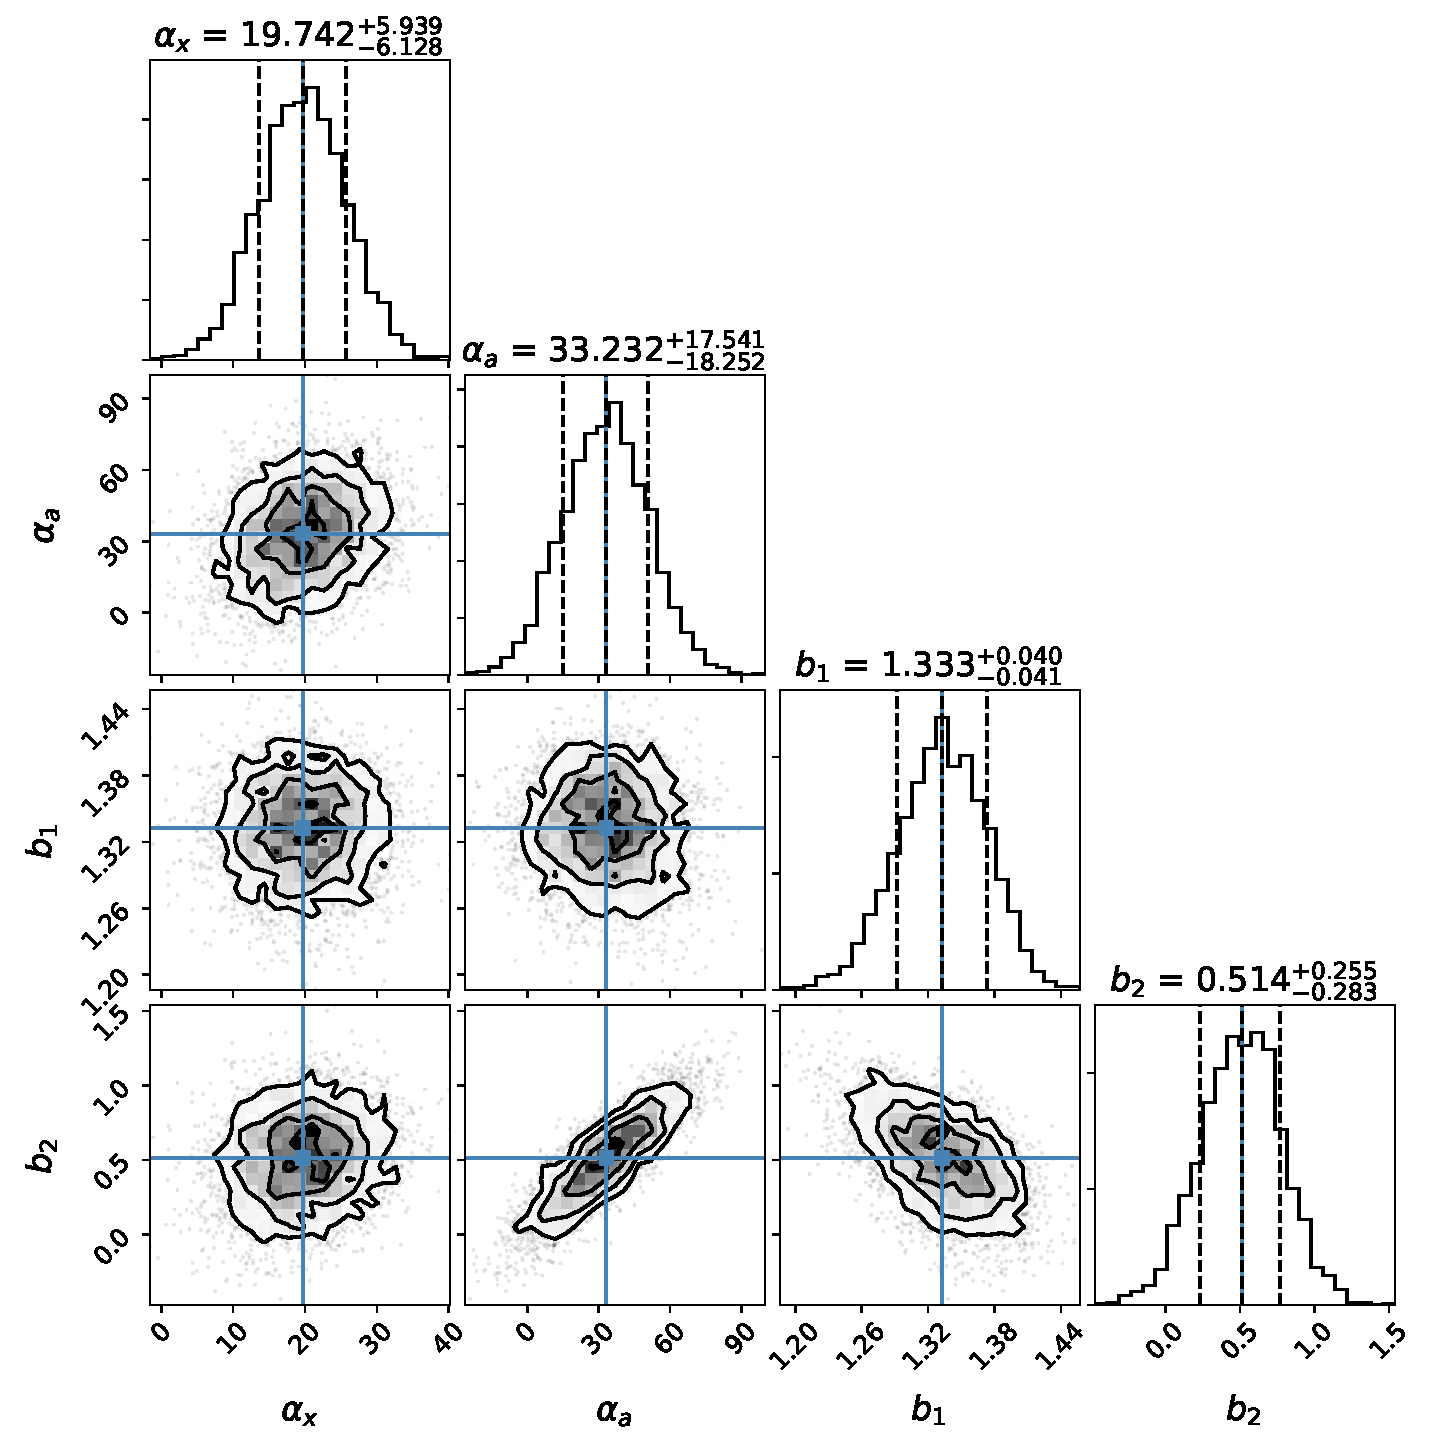
\includegraphics[width=\linewidth,trim={0.4cm 0.2cm 0.2cm 0.2cm},clip]{figures/corner_plot.pdf}
\caption{Marginalized 1D and 2D posterior probability distributions of the parameters. Vertical lines are median values.}
\label{fig:lptmcmc}
\end{figure}

\begin{figure}
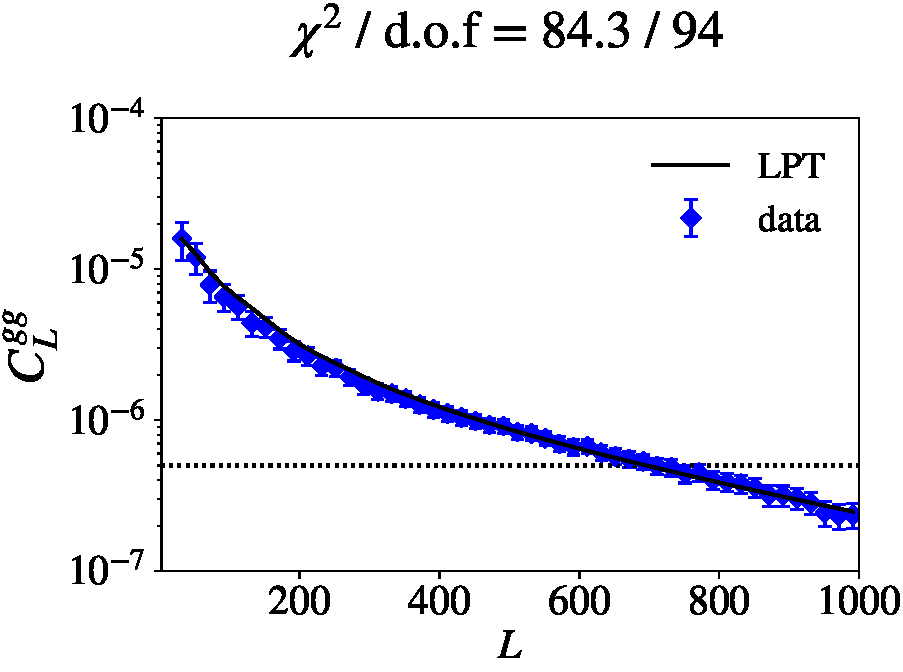
\includegraphics[width=\linewidth]{figures/cl_gg_lpt.pdf}
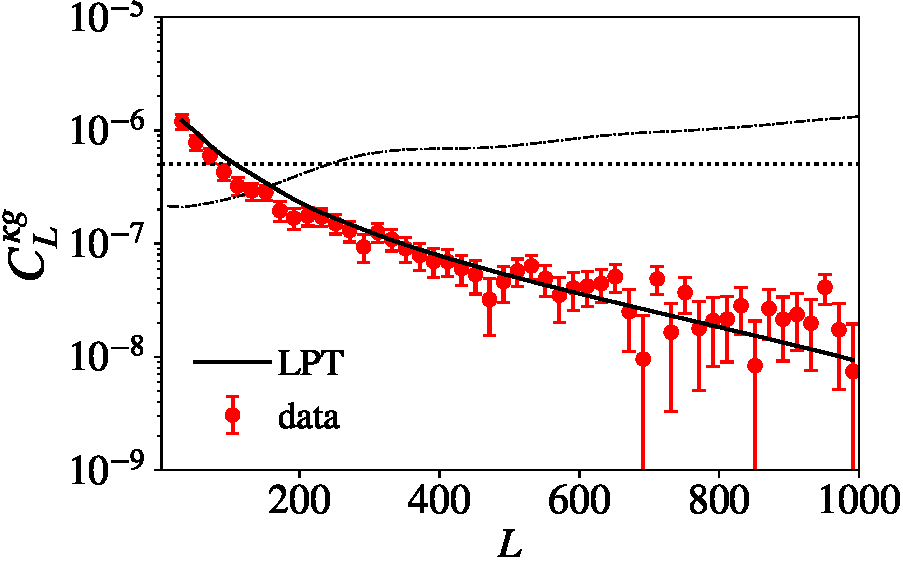
\includegraphics[width=\linewidth]{figures/cl_kg_lpt.pdf}
\caption{The observed galaxy-galaxy (upper plot, blue diamonds) and galaxy-convergence (lower plot, red diamonds) angular power spectra, after subtracting noise and correcting for magnification bias. Solid lines correspond to the predictions from the CLEFT perturbation theory framework using MCMC fitted parameters for $\ell_{\rm max}=1000$ (Table~\ref{tab:lpt_mcmc}). The dotted horizontal line is the galaxy shot noise floor, and the dashed black curve is the lensing noise.}
\label{fig:cl_lptfit}
\end{figure}

We can compare the Lagrangian $b_1$ to the Eulerian bias found in the previous section,
\begin{align}
    b(z_{\rm eff}) &= 1 + b_1(z_{\rm eff}) \\
    &= b(0)/D(z_{\rm eff})
\end{align}
For $z_{\rm eff} = 0.68$, the best fit $b_1 = 1.31$ corresponds to $b(0) = 1.63$, in excellent agreement with the result from our HaloFit model using the photometric redshift distribution. Furthermore, after accounting for the uncertainty associated with photometric versus clustering redshift distributions $\sigma_{b_{\rm gg}} = 0.08$, the effective bias from the perturbation theory model is consistent with the effective bias measured using the clustering $b(z)\phi(z)$ (Table~\ref{tab:halofit_clustering_noevo}). Thus, these two models show excellent consistency with each other, and both are consistent with the assumed bias evolution model.  The LPT-based model provides a statistically acceptable fit to both $C_\ell^{\rm gg}$ and $C_\ell^{\rm \kappa g}$ for our fiducial cosmology, however if one artificially introduces an additional degree of freedom that scales the amplitude of $C_\ell^{\rm \kappa g}$ we find an even better fit is obtained when the model prediction is lowered by 10-20\%.  This is similar to the lower $b_{\rm \kappa g}$ preferred by our HaloFit model, compared to $b_{\rm gg}$.
